% This file was created by matplotlib2tikz v0.7.3.
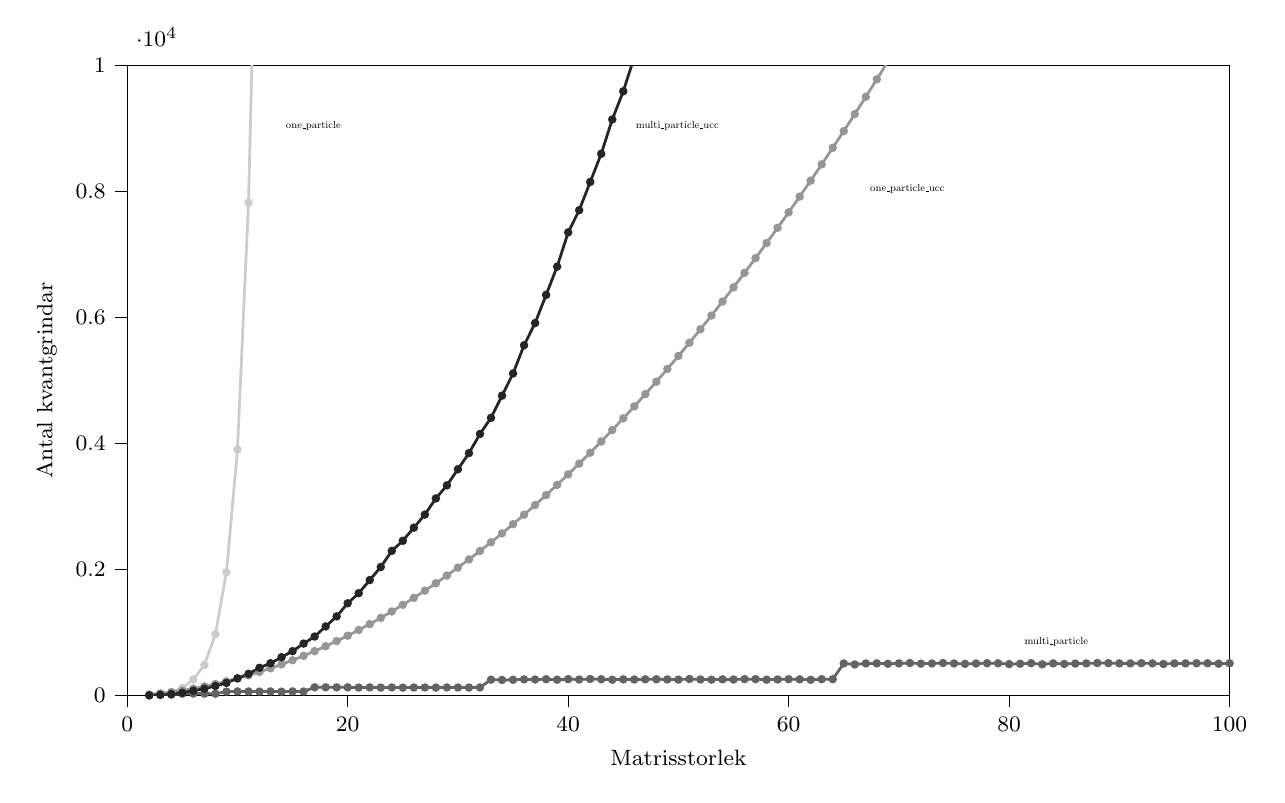
\begin{tikzpicture}

\begin{axis}[
font =\footnotesize,
height=8cm,
minor xtick={},
minor ytick={},
scale only axis,
tick align=outside,
tick pos=left,
width=14cm,
x grid style={white!69.01960784313725!black},
xlabel={Matrisstorlek},
xmin=0, xmax=100,
xtick style={color=black},
xtick={0,20,40,60,80,100},
y grid style={white!69.01960784313725!black},
ylabel={Antal kvantgrindar},
ymin=0, ymax=10000,
ytick style={color=black},
ytick={0,2000,4000,6000,8000,10000}
]
\addplot [line width=1.0pt, white!80.0!black, mark=*, mark size=1, mark options={solid}]
table {%
2 13.4
3 31.4
4 57.6
5 120.4
6 255.6
7 485.8
8 975.2
9 1958.6
10 3903.6
11 7825
12 14882.6
};
\addplot [line width=1.0pt, white!58.82352941176471!black, mark=*, mark size=1, mark options={solid}]
table {%
2 15
3 33
4 55
5 81
6 111
7 145
8 183
9 225
10 271
11 321
12 375
13 433
14 495
15 561
16 631
17 705
18 783
19 865
20 951
21 1041
22 1135
23 1233
24 1335
25 1441
26 1551
27 1665
28 1783
29 1905
30 2031
31 2161
32 2295
33 2433
34 2575
35 2721
36 2871
37 3025
38 3183
39 3345
40 3511
41 3681
42 3855
43 4033
44 4215
45 4401
46 4591
47 4785
48 4983
49 5185
50 5391
51 5601
52 5815
53 6033
54 6255
55 6481
56 6711
57 6945
58 7183
59 7425
60 7671
61 7921
62 8175
63 8433
64 8695
65 8961
66 9231
67 9505
68 9783
69 10065
};
\addplot [line width=1.0pt, white!38.82352941176471!black, mark=*, mark size=1, mark options={solid}]
table {%
2 4
3 13.6
4 13.4
5 30.6
6 31.6
7 31
8 30
9 63
10 65.8
11 64.8
12 63
13 65.8
14 62
15 66
16 64.8
17 131
18 131.4
19 130
20 130.8
21 126.8
22 129.4
23 126.8
24 128.8
25 125.8
26 128.2
27 128.2
28 126.4
29 128.8
30 128
31 127
32 129.2
33 252
34 247.4
35 250
36 256.6
37 254.6
38 259.2
39 251.6
40 260.4
41 254.6
42 263
43 259
44 251.4
45 257.4
46 254.8
47 257.8
48 258.4
49 255.8
50 253
51 263
52 255.4
53 251.8
54 257.6
55 254.6
56 260.6
57 260.8
58 251.6
59 255.2
60 260.4
61 257.2
62 250.6
63 260
64 259.8
65 509.8
66 494
67 510
68 511
69 504
70 510.2
71 516.8
72 506.6
73 509.2
74 516.2
75 509.4
76 503.2
77 509
78 513.2
79 512.2
80 499.6
81 505.6
82 513.4
83 496.2
84 510.8
85 501.8
86 508
87 510.2
88 516.8
89 514.6
90 510.6
91 510
92 513.4
93 510.2
94 501
95 510.2
96 511
97 513
98 512.4
99 505.4
100 513.2
101 511.8
};
\addplot [line width=1.0pt, white!14.50980392156863!black, mark=*, mark size=1, mark options={solid}]
table {%
2 3
3 11
4 25
5 45
6 77
7 109
8 153
9 201
10 273
11 345
12 441
13 513
14 609
15 705
16 825
17 937
18 1097
19 1257
20 1465
21 1625
22 1833
23 2041
24 2297
25 2457
26 2665
27 2873
28 3129
29 3337
30 3593
31 3849
32 4153
33 4409
34 4761
35 5113
36 5561
37 5913
38 6361
39 6809
40 7353
41 7705
42 8153
43 8601
44 9145
45 9593
46 10137
};
\node at (axis cs:14,9000)[
  scale=0.454545454545455,
  anchor=base west,
  text=black,
  rotate=0.0
]{one\_particle};
\node at (axis cs:67,8000)[
  scale=0.454545454545455,
  anchor=base west,
  text=black,
  rotate=0.0
]{one\_particle\_ucc};
\node at (axis cs:81,811.8)[
  scale=0.454545454545455,
  anchor=base west,
  text=black,
  rotate=0.0
]{multi\_particle};
\node at (axis cs:46,9000)[
  scale=0.454545454545455,
  fill=white,
  draw=white,
  line width=0.4pt,
  inner sep=1.1pt,
  anchor=base west,
  text=black,
  rotate=0.0
]{multi\_particle\_ucc};
\end{axis}

\end{tikzpicture}